\documentclass[border=10pt]{standalone}
\usepackage{tikz}
\usetikzlibrary{positioning, shapes.geometric, shapes.symbols, fit, backgrounds, calc}

\begin{document}
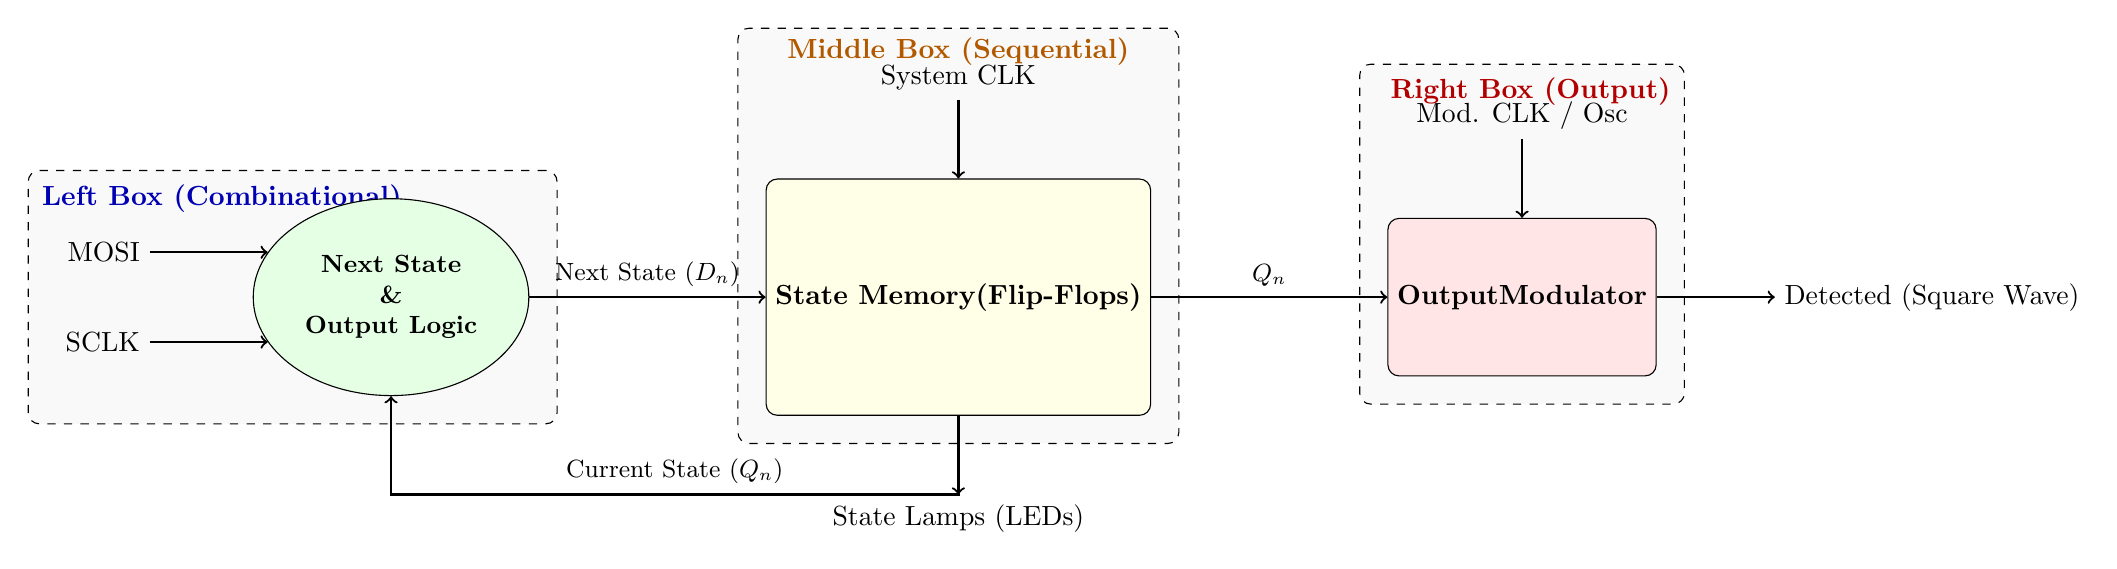
\begin{tikzpicture}
    % Styles
    \tikzset{
        block/.style={rectangle, draw, fill=blue!10, text centered, rounded corners, minimum height=3em, minimum width=4em, font=\bfseries},
        cloud_logic/.style={ellipse, draw, fill=green!10, minimum width=3.5cm, minimum height=2.5cm, align=center, font=\bfseries\small},
        container/.style={draw, dashed, inner sep=1em, rounded corners, fill=gray!5},
        label_text/.style={font=\bfseries\small, align=center}
    }

    % --- Nodes ---

    % Middle Box: State Memory (Flip-Flops)
    \node[block, minimum width=2.5cm, minimum height=3cm, fill=yellow!10] (memory) at (0,0) {State Memory\\(Flip-Flops)};

    % Left Box: Combinational Logic
    \node[cloud_logic, left=3cm of memory] (logic) {Next State\\\&\\Output Logic};

    % Right Box: Output Interface
    \node[block, right=3cm of memory, fill=red!10, minimum width=2.5cm, minimum height=2cm] (output_interface) {Output\\Modulator};


    % --- Connections ---

    % Inputs to Logic
    \node[left=1.5cm of logic.160] (mosi) {MOSI};
    \node[left=1.5cm of logic.200] (sclk) {SCLK};
    \draw[->, thick] (mosi) -- (logic.160);
    \draw[->, thick] (sclk) -- (logic.200);

    % Logic to Memory (Next State D)
    \draw[->, thick] (logic.east) -- node[above, font=\small] {Next State ($D_n$)} (memory.west);

    % Memory to Logic (Feedback Q)
    % We need to route this around
    \draw[->, thick] (memory.south) -- ++(0,-1) -| node[pos=0.25, above, font=\small] {Current State ($Q_n$)} (logic.south);

    % Memory/Logic to Output Interface
    % The prompt implies logic generates "Detected" or "Match" signal first, then modulated
    % Or maybe Q connects to it? Let's assume Logic generates a "Match" signal based on state
    % But wait, "Left Box... contains Output Logic". So Logic -> Match -> Right Box.
    % However, the diagram in Mini Project usually shows Q going to Output Logic.
    % Let's stick to the prompt: "Left Box contains Next-State Logic and Output Logic".
    % So the 'Output Logic' inside the cloud generates the 'Match' condition.
    % Does 'Match' go to Right Box? Yes.
    
    % Let's draw a line from Logic to Right Box, passing *over* Memory or through?
    % A cleaner way: The "Output Logic" part of the Left Box is conceptually what drives the output.
    % But physically, usually Q drives the output decoder. 
    % Let's assume the "Output Logic" is distinct enough to send a signal to the Right Box.
    % OR, maybe the Logic block sends "Match" to the Right Box.
    
    % Alternative interpretation: The "Left Box" is *physically* the combinational chips. 
    % So it takes Q as input. 
    % Let's draw a connection from Logic to Output Interface? 
    % Or simply Q -> Output Interface? 
    % Ref: "Right Box... Handles Detected signal generation". 
    % Ref: "Left Box... Output Logic".
    % This implies: Q -> Left Box (Output Logic) -> Match Signal -> Right Box.
    % This would look messy if Left Box is on the left.
    
    % Let's try to arrange: Logic (Left), Memory (Middle), Output (Right).
    % If Logic generates Match, it has to pass through/around Memory?
    % Maybe the "Output Logic" is a separate block physically, but classified as "Left Box"?
    % Let's clarify the feedback loop first. Logic -> D -> Memory -> Q -> Logic.
    % AND Memory -> Q -> output_interface?
    % If "Output Logic" is in Left Box, maybe it's purely Next State Logic + Mealy/Moore Output decoding?
    % If Moore: Output depends on Q. Q -> Logic -> Match.
    % If Mealy: Output depends on Q + Inputs.
    % Let's assume Moore/Mealy combo.
    % Connection: Capture "Match" from logic? 
    % Let's draw: Memory -> Output Interface (Q bus). This is standard.
    % Then Output Interface contains "Logic" to detect specific state?
    % BUT prompt says "Left Box" contains "Output Logic".
    % Let's compromise: Draw a "Match" line from the Logic Cloud appearing to go to the Right Box.
    % Better: The Feedback path (Q) is available to everyone.
    % Let's tap off the Feedback path to the Right Box.
    
    \draw[->, thick] (memory.east) -- node[above, font=\small] {$Q_n$} (output_interface.west);
    
    % Clock to Memory
    \node[above=1cm of memory] (clk) {System CLK};
    \draw[->, thick] (clk) -- (memory.north);

    % Output Interface Inputs
    % Needs modulation clock?
    \node[above=1cm of output_interface] (mod_clk) {Mod. CLK / Osc};
    \draw[->, thick] (mod_clk) -- (output_interface.north);

    % Final Output
    \node[right=1.5cm of output_interface] (detected) {Detected (Square Wave)};
    \draw[->, thick] (output_interface.east) -- (detected);

    % State Lamp
    \node[below=1.0cm of memory] (lamps) {State Lamps (LEDs)};
    \draw[->, thick] (memory.south) ++(0,-0.5) -- (lamps.north);


    % --- Containers (Boxes) ---
    
    \begin{scope}[on background layer]
        % Left Box
        \node[container, fit=(logic) (mosi) (sclk), label={[anchor=north west, font=\bfseries\color{blue!70!black}, inner sep=5pt]north west:Left Box (Combinational)}] (box_left) {};
        
        % Middle Box
        \node[container, fit=(memory) (clk), label={[anchor=north, font=\bfseries\color{orange!70!black}]north:Middle Box (Sequential)}] (box_mid) {};
        
        % Right Box
        \node[container, fit=(output_interface) (mod_clk), label={[anchor=north east, font=\bfseries\color{red!70!black}, inner sep=5pt]north east:Right Box (Output)}] (box_right) {};
    \end{scope}

\end{tikzpicture}
\end{document}
